\documentclass[11pt]{article}
\usepackage[a4paper,top=3cm,bottom=3cm,left=2cm,right=2cm]{geometry}
%\usepackage{geometry}                % See geometry.pdf to learn the layout options. There are lots.
\geometry{letterpaper}                   % ... or a4paper or a5paper or ... 
%\geometry{landscape}                % Activate for for rotated page geometry
%\usepackage[parfill]{parskip}    % Activate to begin paragraphs with an empty line rather than an indent
\usepackage{graphicx}
\usepackage{amssymb}
\usepackage{epstopdf}
\usepackage{bashful}
\usepackage{amsmath}
\usepackage[english]{babel}
\usepackage{hyperref}
\DeclareGraphicsRule{.tif}{png}{.png}{`convert #1 `dirname #1`/`basename #1 .tif`.png}

\title{CS281 Status Update \\
	\large Scalable Signal Region Identification with applications to the ATLAS $W^\pm W^\pm W^\pm$ Analysis}
\author{Nicol\`o Foppiani, Jonah Philion, Baojia(Tony) Tong}
\date{}   

% Activate to display a given date or no date

\begin{document}
\maketitle

\centering
\href{https://github.com/tongbaojia/cs281_mlphys}{https://github.com/tongbaojia/cs281\_mlphys}

\renewcommand{\abstractname}{Draft of the final abstract}
\begin{abstract}
In experimental particle physics new phenomena is observed and eventually discovered by looking for statistically significant deviations in the count data over the space of the features which are experimentally measured.\\
Therefore, this projects aims to develop general strategies to identify signal regions in high background parameter space. This can be naively done by cutting the space in baskets and using the basket with the largest significance. However, thanks to the grown of the computational power, it is nowadays possible to exploit Machine Learning. Several techniques have been studied in order to train classifiers between signal and background, such as Decision Trees and Neural Networks. Furthermore, the problem of maximizing the statistical significance instead of classifying signal and background has been investigated.\\
The whole project has been developed by studying the simulated dataset of $W^\pm W^\pm W^\pm$ events collected by the ATLAS detector. The results are promising, showing important improvements with respect to the cut-based analysis. These methods will be adopted in the official ATLAS analysis.
\end{abstract}

\paragraph{Problem Statement}
In particle physics analysis, there is in general some ``signal" process that generates data simultaneously as ``background" processes generate similar looking data. Given unlabeled data from all processes, our goal is to determine the likelihood that the signal process exists.\\
To generate data $\{x_i\}_N$ lying in $\mathbb{R}^n$, we associate to the signal process a smooth function $s: \mathbb{R}^n \rightarrow \mathbb{R}_{> 0}$ and to the background process $b: \mathbb{R}^n \rightarrow \mathbb{R}_{> 0}$ such that for any volume $V \subset \mathbb{R}^n$, the number of background events in this region $n_{bkg}(V)$ and the number of signal events in this region $n_{sig}(V)$ can  be modeled as 

\[ n_{bkg}(V) \sim \text{Pois} \left( \int_V b \right)\]
\[n_{sig}(V) \sim \text{Pois} \left( \int_V s \right) \]

\paragraph{}
The data is generated from these Poisson processes. We can then determine the likelihood of the existence of the signal process by choosing regions of our parameter space $\{V_j\}$ then comparing the number of events observed in these regions to the values $\{n_{bkg}(V_i)\}$ and $\{n_{sig}(V_i) + n_{bkg}(V_i)\}$. For the case of large $N$, we can approximate the Poisson distribution as Gaussian. For a region with $O$ observed events, the significance is then
\begin{equation}
Significance \approx \frac{O-n_{bkg}(V)}{\sqrt{n_{bkg}(V)}}
\label{significance}
\end{equation}

\paragraph{}
We have simplified our problem to determining the set $\{V_i\}$ of regions of parameter space which will maximize the definition of significance in Equation~\ref{significance}.\\
It is noteworthy to point out that this problem is not trivial. In fact, the simplest approach is to try to classify signal and background: this means to estimate the probability to be signal for each value of the experimental features. Regions with larger fractions of signal events will be more likely to be significant. However this is not always the case, and a proper optimization of the significance should be done.\\
A second caveat is due to the uncertainty on the significance: we want to identify regions in which the significance is large with small fluctuations. For instance, optimizing the significance might bring to rely on regions in which we have one expected signal event and $10^{-3}$ background event: this region would be very significant but not reliable, since the \textit{uncertainty} on the significance will be large.

\paragraph{Baselines}
Since our goal is to determine volumes of parameter space which maximize the significance, one baseline is to take the volume to be the entire parameter space. The metrics for this approach are summarized in table~\ref{baselines}.

In particle physics a significance greater than $3\sigma$ is required by the community to claim an observation, and a significance larger than $5\sigma$ in order to claim a discovery. The observed significance in our dataset is $0.517\sigma$: this is much smaller than what request for observing this rare physical process. Thus, this puts a strong motivation in applying new techniques in order to enlarge this value.

A description of the data used in this analysis is shown in table~\ref{data}. This table illustrates the various features which have been selected, stressing also if they are continuous or categorical variables.
In the end, it will also be of interest to try to reduce the variables to the subset of the most significant ones. 

\begin{table}[!htbp]
\begin{center}
\begin{tabular}{|l|l|l|l|}

  %\hline
  \cline{2-4}
  \multicolumn{1}{c|}{} & $n_{sig}$ & $n_{bkg}$ & $n_{sig}/\sqrt{n_{bkg}}$ \\
  \hline
  No Cuts & 47.09 & 8288.18 & 0.517$\sigma$ \\
  \hline
\end{tabular}
\caption{Baseline measurements. $n_{sig}$ is the weighted sum of all signal events, $n_{bkg}$ is the weighted sum of all background events, and $S/\sqrt{B}$ is our metric for the significance. The objective is to maximize the significance, resulting in some value larger than the 3$\sigma$ limit.}
\label{baselines}
\end{center}
\end{table}

\begin{table}[!htbp]
\begin{center}
\begin{tabular}{|c|c|c|}

  \hline
  Variable Name & Description & Type \\
 \hline
 \hline
$ j^0_m $ & Invariant mass of the most energetic jet & continuous\\
\hline
$ j^0_{p_T} $ & Transverse momentum of the most energetic jet & continuous\\
\hline
$ j^0_{\eta} $ & Pseudorapidity of the most energetic jet & continuous\\
\hline
$ j^0_{\phi} $ & Azimuthal angle of the most energetic jet & continuous\\
\hline
$ l^0_m $ & Invariant mass of the highest $p_T$ lepton & continuous\\
\hline
$ l^0_{p_T} $ & Transverse momentum of the highest $p_T$ energetic lepton & continuous\\
\hline
$ l^0_{\eta} $ & Pseudorapidity of the  highest $p_T$ lepton & continuous\\
\hline
$ l^0_{\phi} $ & Azimuthal angle of the highest $p_T$ lepton & continuous\\
\hline
$ l^0_c $ & Charge of the  highest $p_T$ lepton & categorical\\
\hline
$ l^0_{isEl} $ & 1 if the most energetic lepton is an electron, 0 for muon & categorical\\
\hline
$ l^1_m $ & Invariant mass of the second-to-most energetic lepton & continuous\\
\hline
$ l^1_{p_T} $ & Transverse momentum of the second-to-most energetic lepton & continuous\\
\hline
$ l^1_{\eta} $ & Pseudorapidity of the second-to-most energetic lepton & continuous\\
\hline
$ l^1_{\phi} $ & Azimuthal angle of the second-to-most energetic lepton & continuous\\
\hline
$ l^1_c $ & Charge of the second-to-most energetic lepton & categorical\\
\hline
$ l^1_{isEl} $ & 1 if the second-to-most energetic lepton is an electron, 0 for muon & categorical\\
\hline
$ l^2_m $ & Invariant mass of the third-most energetic lepton & continuous\\
\hline
$ l^2_{p_T} $ & Transverse momentum of the third-most energetic lepton & continuous\\
\hline
$ l^2_{\eta} $ & Pseudorapidity of the third-most energetic lepton & continuous\\
\hline
$ l^2_{\phi} $ & Azimuthal angle of the third-most energetic lepton & continuous\\
\hline
$ l^2_c $ & Charge of the third-to-most energetic lepton & categorical\\
\hline
$ l^2_{isEl} $ & 1 if the third-to-most energetic lepton is an electron, 0 for muon & categorical\\
\hline
$ met_{p_T} $ & Transverse momentum of the missing transverse energy & continuous\\
\hline
$ met_{phi} $ & Azimuthal angle of the missing transverse energy & continuous\\
\hline
$ weight $ & event weight, normalization to the correct data size, and kinematic corrections & continuous\\
\hline
$ cl $ & The physics process that generated event. & categorical\\
\hline
$ is_{sig} $ & 1 if signal, 0 if background. & categorical\\
\hline
\end{tabular}
\caption{Feature Space. We measure $cl$, $is_{sig}$, and $weight$ only in simulation. We measure all other variables in real data and in simulation. Our general approach to train classifiers to predict $is_{sig}$ given the jet and lepton features.}
\label{data}
\end{center}
\end{table}




\paragraph{Approaches}
\begin{enumerate}

\item {\bf Physics Motivated Cuts}
Cuts from the most recent analysis paper. This will be the baseline that we try to achieve and beat.

\item {\bf Naive Classification}
The first approach is to train a classifier $x \rightarrow y$ where $x$ is a list of kinematic and categorical variables and $y$ is the binary label: $0$ for background and $1$ for signal. The loss function used in this case is the cross entropy, weighted with the relative weights of the events, in order to obtain the correct mixture of events predicted by the theory.\\
Three approaches has been pursued:
\begin{itemize}
    \item Logistic regression (using Pytorch)
    \item Neural network classifier (using Pytorch)
    \item Boosted decision trees (using XGBoost)
\end{itemize}

\item {\bf Category Specific Classification}
We factor the probability that an event is a signal as 
\[p(event.is_sig == 1) = p(event.isSig == 1|x_{categorical}) * p(event.isSig == 1|x_{continuous})\]
We model the first probability as a categorical distribution with probabilities given by 
$$p(event.isSig == 1|x_{categorical}) = \frac{\sum 1_{category, signal}w}{1_{category}w}$$
We model the second probability using XGBClassifier on a small parameter grid with 3-fold cross validation.\\
At test time, for every event, we calculate the probabilities $p(event.is_sig == 1)$. We then make a histogram of $p$ and evaluate the significance on a combination of these bins. We calculated the significance for train and test data: they are shown in figure ~\ref{fig:train} and figure ~\ref{fig:test}, respectively. The raw values are shown in table ~\ref{tab:smallsig}.



\begin{table}[!htbp]
\begin{center}
\begin{tabular}{|l|l|l|l|}
\cline{2-4}
\multicolumn{1}{c|}{} & $n_{bkg}$ & $n_{sig}$ & $n_{sig}/\sqrt{n_{bkg}}$\\
\hline
train & 44.271 & 10.995 & $1.652\sigma$\\
\hline
test & 41.478 & 10.994 & $1.707\sigma$\\
\hline
\end{tabular}
\caption{Category Specific Classification Results. The significance is 328$\%$ better than the baseline. We will calculate the variance on this test error with bootstrapping.}
\end{center}
\label{tab:smallsig}
\end{table}


\begin{figure}[!htbp]
    \begin{center}
    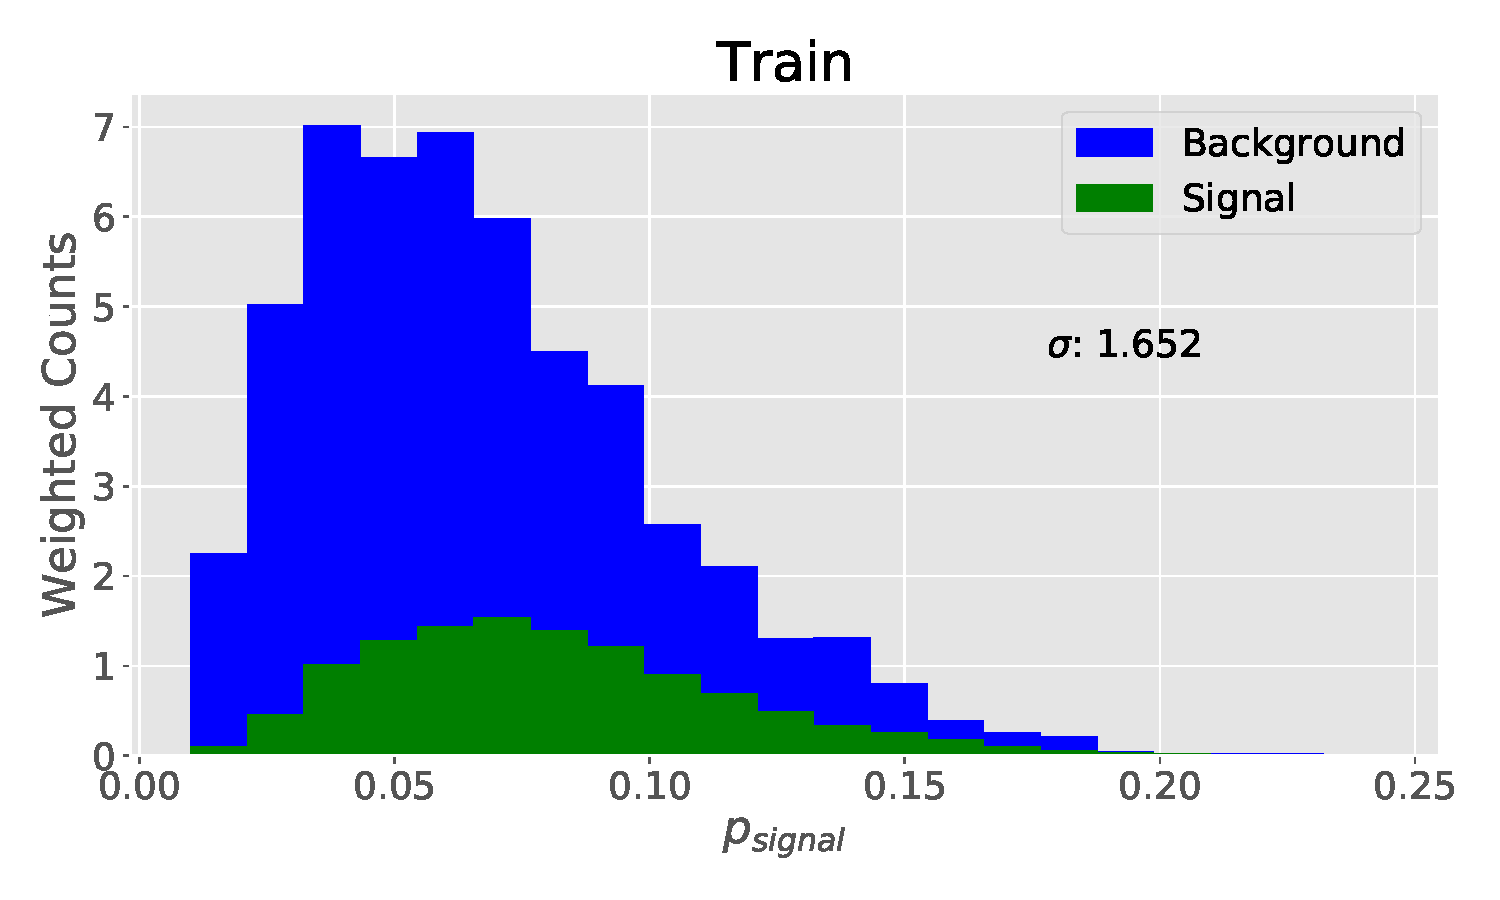
\includegraphics[width=150mm]{train.pdf}
    \caption{Category Specific Classification. Histograms of estimated probabilities for all events. Only events with $p>.01$ are included in this plot because the background dominates in the region $p<.01$. The significance is computed over bins with $p>0.0322$. We make this decision based on the training set distribution only.}
    \label{fig:train}
    \end{center}
\end{figure}

\begin{figure}
    \begin{center}
    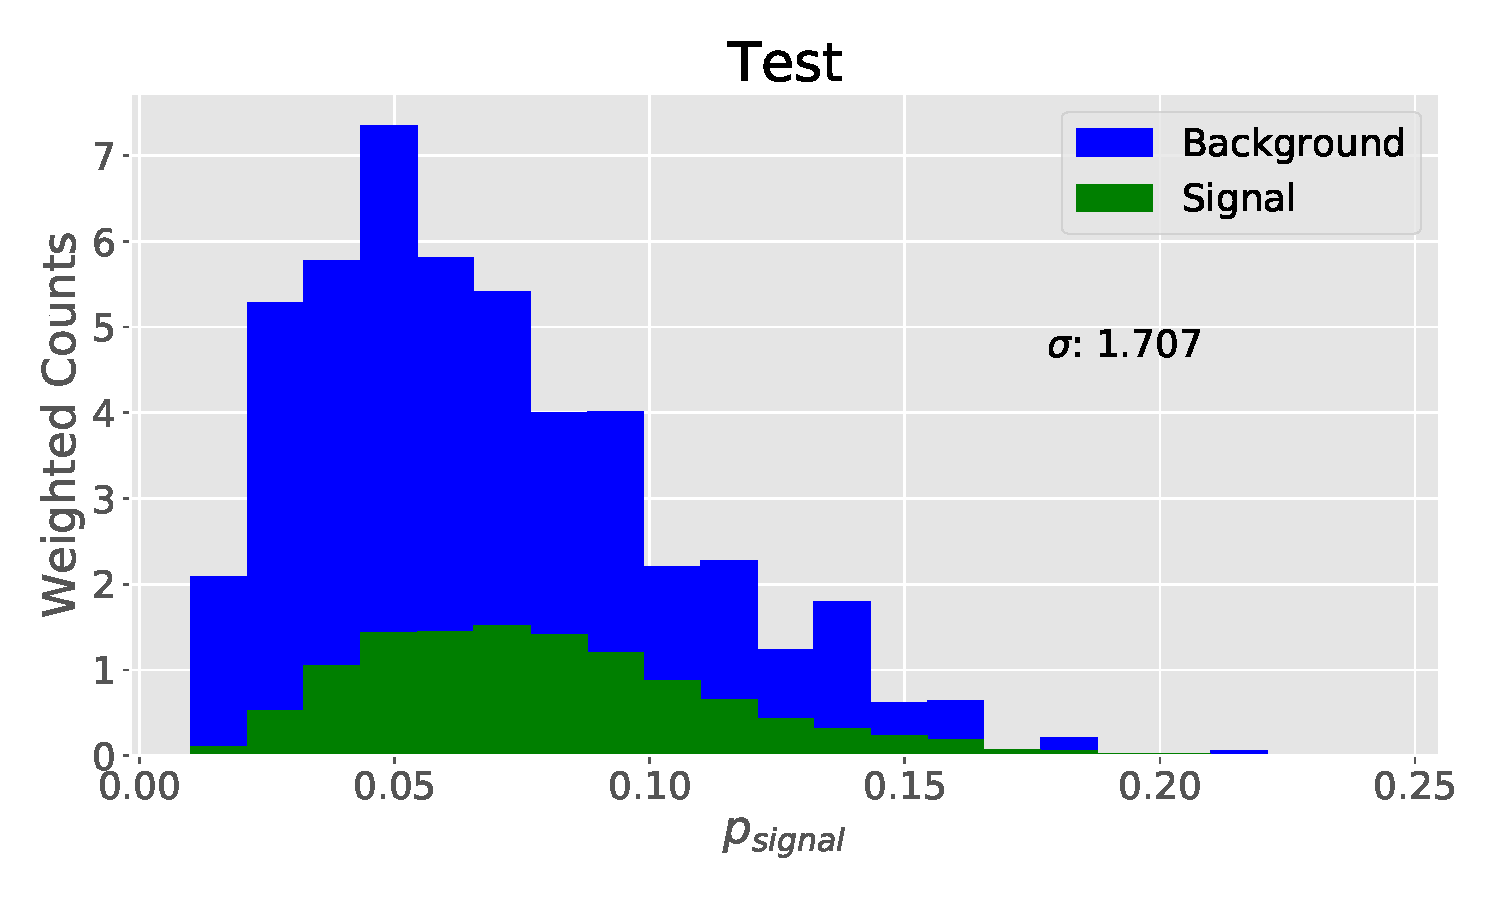
\includegraphics[width=150mm]{test.pdf}
    \centering
    \caption{Category Specific Classification. The equivalent graph to ~\ref{fig:train} but over the test set. The significance is about the same in the test set as it is in the train set. We'll have to run the algorithm on different random train/test partitions (bootstrapping) to get a sense of the variance of this test $\sigma$.}
    \label{fig:test}
    \end{center}
\end{figure}




\item {\bf Loss function containing significance}
Optimizing the crossentropy lets us make inference on the probability to be signal for each value of the features. However, the goal is not to have the greatest possible separation in two classes, but to obtain the highest significance for the discovery. The problem of optimizing an analysis in order to maximize the significance is hard and few studies are present in the scientific literature.\\
The most naive approach is to make the significance differentiable and optimize it as a loss function. This has not led to any exceptional result so far.
Additionally we are also trying to implement a more robust loss function, which we can maximize obtaining the highest significance.

\end{enumerate}

It is expected to summarize together the results by the end of November.
\end{document}  